\documentclass[a4paper,openright,12pt]{article}
\usepackage[utf8]{inputenc}
\usepackage{graphicx} 
\usepackage{subfigure}
\usepackage{caption}
\usepackage{subcaption}
\usepackage[mathscr]{eucal}
\usepackage{titling}
\usepackage{float}
\usepackage{amsmath}
\usepackage{afterpage}
\usepackage{vmargin}
\usepackage[spanish]{babel}
\usepackage{eurosym} 
\usepackage{multirow} 
\usepackage{cite}
\usepackage{url}

\setpapersize{A4}   %  DIN A4
\setmargins{3cm}    % margen izquierdo
{3.5cm}             % margen superior
{15cm}              % anchura del texto
{22.5cm}            % altura del texto
{10pt}              % altura de los encabezados
{1cm}               % espacio entre el texto y los encabezados
{0pt}               % altura del pie de página
{2cm}               % espacio entre el texto y el pie de página

\begin{document}

\begin{titlepage}
    \begin{center}
        \vspace*{-1in}
        \begin{figure}[htb]
            \begin{center}
                
\includegraphics[width=8cm]{udc.eps}
            \end{center}
        \end{figure}

        \vspace*{1in}
        PROGRAMACIÓN DE SISTEMAS 22/23 Q1\\
        \begin{figure}[htb]
            \begin{center}
                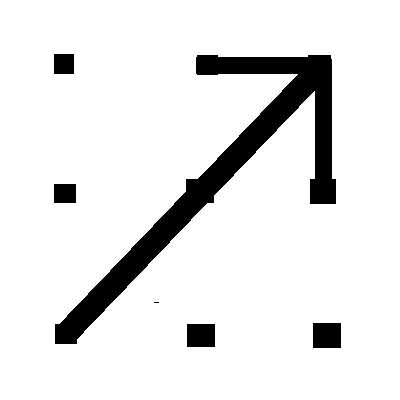
\includegraphics{icon.png}
            \end{center}
        \end{figure}
        \vspace*{1in}
        \begin{Large}
            \textbf{MallaVectores} \\
        \end{Large}
        
        \vspace*{3in}
        
        \begin{large}
            \raggedleft
            \textbf{Autores:}Iago Valeiro Castrillón \\
            Alejandro Dopazo López \\
            Alberto Ferreiro Campello \\
            \textbf{Fecha:}\textit{A Coruña, 19 Diciembre 2022} \\
        \end{large}
        
    \end{center}
\end{titlepage} 

\newpage

\addtocontents{toc}{\hspace{-7.5mm} \textbf{Capítulos}}
\addtocontents{toc}{\hfill \textbf{Página} \par}
\addtocontents{toc}{\vspace{-2mm} \hspace{-7.5mm} \hrule \par}

\pagenumbering{empty}

\tableofcontents

\vspace{5cm}

\begin{flushright}
    \begin{table}[hbtp]
        \begin{center}
        
            \caption{Tabla de versiones.}
            \label{tabla:versiones}
            \small
            \vspace{1ex}
            
            \begin{tabular}{|c|c|l|}
                \hline
                Versión & Fecha & Autor \\
                \hline \hline
                x & y & \\ \hline
                x & y & \\ \hline
                x & y & \\ \hline
            \end{tabular}
            
        \end{center}
    \end{table}
\end{flushright}

\newpage
\pagenumbering{arabic}


%%%%%%%
%%%%%%%
\section{Introducción}\label{cap.introduccion}
La aplicación propuesta consiste en un editor de imágenes vectoriales para dispositivos móviles Android, inicialmente sería para la creación de iconos y basaría su funcionamiento en la interconexión de puntos en una malla cuadriculada, además llevaría integrado un sistema de guardado local mediante una base de datos SQL, y la posibilidad de guardar las imágenes exportadas en la nube con Firebase.

%%
\subsection{Objetivos}
\begin{enumerate}
    \item Principal:
    \begin{itemize}
        \item Creación de imágenes vectoriales a partir de puntos, líneas y curvas.
    \end{itemize}

    \item Secundarios:
    \begin{itemize}
        \item Exportación de las imágenes a formatos de archivo habituales como \\
        .svg~\cite{SVG} que permitan compartirlas con otros usuarios.
        \item Manejo de los cambios en las imágenes mediante un sistema de guardado local en base de datos SQL~\cite{SQL}.
    \end{itemize}
\end{enumerate}

Las dependencias son las especificadas en la sección \emph{Funcionalidades}

%%
\subsection{Motivación}
Crear una herramienta con la que poder experimentar fácil y cómodamente con gráficos vectoriales, se trata de un tema de especial interés dada la relativa carencia de herramientas destinadas a estos fines.
Es aplicable para, por ejemplo, el diseño de recursos para aplicaciones gráficas, principalmente iconos.

%%
\subsection{Trabajo relacionado}
\begin{itemize}
    \item Dot Matrix~\cite{Dot_Matrix}, se trata de la aplicación original que dio pié a este proyecto, consta de un editor de iconos desarrollado para Linux por un equipo de 10 personas en el lenguaje de programación Vala~\cite{Vala}. Se puede ver en la figura \ref{fig:trabajo_relacionado}.\subref{fig:dot_matrix}.
    \item Gráficos Vectoriales~\cite{Graficos_Vectoriales} en este caso se trata de una aplicación Android similar a la que se plantea, es bastante completa y se oferta como conversor de archivos .png y .jpg a .svg. Se puede ver en la figura \ref{fig:trabajo_relacionado}.\subref{fig:graficos_vectoriales_app}.
\end{itemize}

\begin{figure}
    \hfill
    \subfigure[Dot Matrix\label{fig:dot_matrix}]{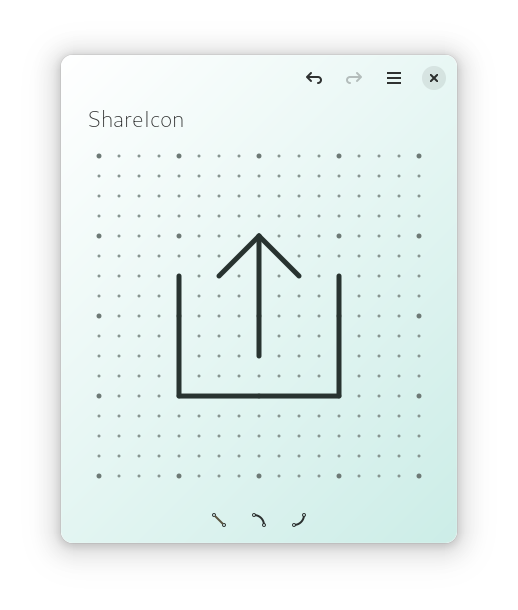
\includegraphics[width=7.5cm]{imagenes/dot_matrix_original.png}}
    \hfill
    \subfigure[Graficos Vectoriales\label{fig:graficos_vectoriales_app}]{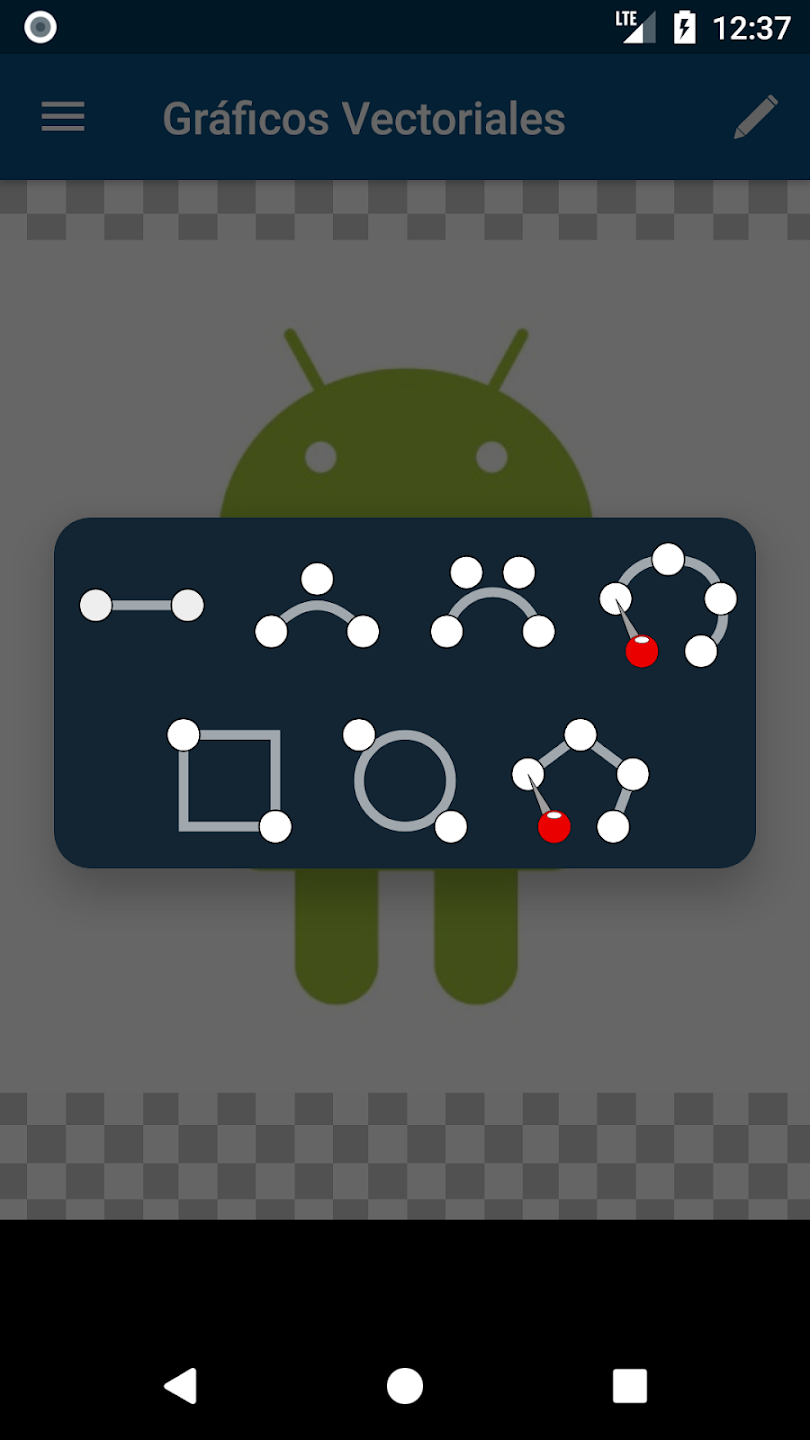
\includegraphics[width=7cm]{imagenes/graficos_vectoriales_app.png}}
    \hfill
    \caption{Ejemplos de aplicaciones similares.}
    \label{fig:trabajo_relacionado}
\end{figure}

%%%%%%%
%%%%%%%
\section{Análisis de requisitos}
\begin{itemize}
    \item La aplicación debe ser capaz de permitir al usuario realizar dibujos utilizando gráficos vectoriales que permitan ser redimensionados sin perder calidad.
    \item Dichos dibujos pueden incluir líneas rectas y curvas, la aplicación que se desarrolle debe dar soporte a ambas.
    \item Con el objetivo de facilitar el proceso de dibujado, si dos vértices están muy próximos estos deberían unirse de forma automática. Dicho de otro modo, los puntos de inicio y fin de cada línea deben ser fijos, dispuestos en una cuadrícula de puntos.
    \item Se espera que la aplicación incluya una opción habitual de los editores de imágenes como es "deshacer".
    \item La aplicación debe permitir exportar los dibujos a formatos de archivo habituales.
    \item Dichos archivos deben poderse compartir.
\end{itemize}

%%
\subsection{Funcionalidades}
\subsubsection{Creación de imágenes vectoriales}
Se pueden disponer los siguientes elementos en la pantalla:
\begin{itemize}
	\item Líneas rectas.
	\item Curvas de Bézier~\cite{Curvas_de_Bezier} cúbicas.
	\item Curvas de Bézier cuadráticas.
\end{itemize}

Cada tipo de elemento tiene un modo asociado, que se puede seleccionar mediante la barra de botones de la actividad principal.
Los modos están identificados por iconos que identifican a las curvas cuadráticas y cúbicas.

El modo actual se muestra al principio de la barra de botones.

Las líneas rectas se dibujan arrastrando entre los dos puntos que vayan a definirla.

Las curvas se definen pulsando primero en cada punto de la recta y luego en sus puntos de control.
Las curvas cuadráticas tienen un punto de control y las cúbicas dos.

\subsubsection{Exportación a ficheros}
Depende de la funcionalidad \emph{Creación de imágenes vectoriales}.
Las imágenes generadas se pueden exportar a ficheros externos en formato svg. El formato usado se ceñirá a la especificación SVGTiny~\cite{SVGTiny} excepto las funciones de text, al igual que los VectorDrawable de Android~\cite{VectorDrawable}.

%%

\subsection{Sistema de guardado local}
Se implementará un sistema de guardado local mediante una base de datos SQL, esta guardará cada línea del dibujo en formato String lo que permitirá realizar las siguientes acciones:
\begin{itemize}
    \item Deshacer/rehacer la última acción.
    \item Eliminar un trazo específico.
    \item Guardar distintos dibujos.
    \item Exportar un dibujo concreto a SVG para su guardado en la nube y/o compartir con otras apps.
\end{itemize}

%%

\subsection{Guardado automático de los ficheros}
La base de datos local se actualizará cada vez que se añada un nuevo trazo, además habrá un servicio en segundo plano que convertirá las imágenes creadas a un fichero SVG y lo subirá a Firebase~\cite{Firebase} de forma automática cada cierto tiempo. 

Esta funcionalidad estará inicialmente desactivada y se podrá activar y configurar desde la propia aplicación.

%%
\subsection{Prioridades}
\begin{enumerate}
    \item Creación de imágenes vectoriales.
    \item Guardado local.
    \item Edición de imágenes.
    \begin{itemize}
        \item Deshacer.
        \item Rehacer.
        \item Seleccionar y eliminar un trazo.
    \end{itemize}
    \item Exportación a ficheros.
    \item Compartir a otras apps.
    \item Integración con Firebase.
    \item Guardado automático en la nube.
\end{enumerate}



%%%%%%%
%%%%%%%
\section{Planificación inicial}

%%
\subsection{Iteraciones}\label{iteraciones}
Primera iteración: Implementación de la funcionalidad \emph{Exportación a ficheros} y \emph{Creación de imágenes vectoriales}.

Segunda iteración: Implementación de la funcionalidad \emph{Exportación a ficheros}.

Tercera iteración: Implementación de la funcionalidad \emph{Guardado en base de datos}.

Cuarta iteración: Implementación de la funcionalidad \emph{Guardado automático de los ficheros}.

Posiblemente otras iteraciones, dependiendo del curso del desarrollo: Expansión de funcionalidades; por ejemplo, posibilitar la interacción con otros elementos del estándar SVGTiny~\cite{SVGTiny}, como rellenos y colores, o posibilitar la exportación a distintos formatos.


%%

\subsection{Responsabilidades}
Iago Valeiro Castrillón: 
\emph{Creación de imágenes vectoriales}, 
\emph{Exportación a ficheros}, 
\emph{Guardado automático de los ficheros} e 
\emph{Guardado en base de datos}.

Alejandro Dopazo López:
\emph{Creación de imágenes vectoriales}, 
\emph{Exportación a ficheros}, 
\emph{Guardado automático de los ficheros} e 
\emph{Guardado en base de datos}.

Alberto Ferreiro Campello:
\emph{Creación de imágenes vectoriales}, 
\emph{Exportación a ficheros}, 
\emph{Guardado automático de los ficheros} e 
\emph{Guardado en base de datos}.


%%
\subsection{Hitos}
Primer entregable: primera iteración implementada. Pruebas de las funcionalidades implementadas.

Segundo entregable: segunda iteración implementada. Pruebas de las funcionalidades implementadas.

Tercer entregable: tercera iteración implementada. Pruebas de las funcionalidades implementadas.

Entregable final: Pruebas de integración y de usabilidad. Revisión de las iteraciones anteriores.

%%
\subsection{Incidencias}
\begin{itemize}
    \item El proyecto transcurre demasiado rápido/despacio:
\end{itemize}
Se añadirán o quitarán iteraciones al proyecto de acuerdo a lo especificado en la sección \ref{iteraciones}. Los hitos y los entregables se ajustarán apropiadamente.

%%


%%%%%%%
%%%%%%%
\section{Diseño}
%%
\subsection{Arquitectura}
Se utilizará la arquitectura Clean Code~\cite{CleanCode} basada en el patrón de diseño model view controller o MVC~\cite{MVC}.

\subsubsection{Actividad principal}
MainActivity, con una barra con botones para seleccionar los modos de dibujo una Vistamalla que muestre la imagen en sí y responda a las acciones y un menú de opciones con:
\begin{itemize}
	\item Exportación de la imagen actual a un fichero.
    \item Conectarse a Firebase para el sistema de guardado en la nube.
    \item Lanzar la actividad Ajustes.
\end{itemize}
%%

\subsubsection{Vistamalla}
La vista muestra una malla de puntos y las formas dibujadas por el usuario.

Gestiona su propia interacción con el usuario.

Envía los trazos a base de datos.
%%

\subsubsection{Actividad Ajustes}
Muestra un sistema de login para utilizar los servicios de Firebase, así como una entrada para cambiar la frecuencia con la que se guarda automáticamente la imagen actual, y un botón para habilitar el servicio GuardadoAutomatico.

%%

\subsection{Persistencia}
Se almacenarán las imágenes en una base de datos SQL. Además se almacenarán los ajustes del servicio de guardado automático en un fichero local "SharedPreferences".

%%

\subsection{Vista}
Una actividad principal mostrando un menú con las acciones que se pueden realizar sobre la imagen actual. La actividad contiene el fragmento con la malla de puntos.

Desde el menú de la actividad principal se puede navegar a la actividad de ajustes.

En la actividad de ajustes se muestra una entrada para cambiar la frecuencia con la que se guarda automáticamente la imagen actual y un botón para deshabilitar el servicio de guardado automático.

%%

\subsection{Comunicaciones}
Las imágenes se guardan en formato String en la base de datos local (un nombre/id y múltiples path, uno por cada trazo).
Para enviar una imagen, se extrae de la base de datos y se convierte a SVG, tras la conversión se envía mediante un intent a otras apps, o a la base de datos online en Firebase.

%%

\subsection{Sensores}
No se debería usar ninguno explícitamente aparte de la entrada por la pantalla táctil.
%%

\subsection{Background}
\subsubsection{Servicio GuardadoAutomatico}
Mientras el usuario va haciendo su diseño se irán guardando sus 
avances en local, además si el usuario lo desea, puede activar el sistema de guardado en la nube en Firebase.

El guardado automático en la nube sucederá mediante el servicio GuardadoAutomatico. Éste sucederá cada vez que pase un período definido en la actividad Ajustes.

%%

\section{Avances sobre el entregable anterior}
\subsection{Diseño}
Ya que la librería para trabajar con Git no ofrece soporte para Android, y no se han encontrado alternativas funcionales, se ha quitado del diseño a favor de Firebase.

%%

\subsection{Avances}
Se ha añadido el icono a la aplicación.
Se ha cambiado el modo de selección de línea de texto a iconos.
Se ha implementado la arquitectura Clean Code para el acceso a base de datos.

%%

\subsection{Hitos}
Actualmente la aplicación permite realizar dibujos mediante distintos tipos de trazos, para probar el modo dibujo, simplemente se instala en un dispositivo o emulador y:
\begin{itemize}
    \item Para dibujar líneas rectas, seleccionamos el modo línea y observamos que ha cambiado la previsualización de herramienta seleccionada, a continuación tocamos donde queremos que inicie y arrastramos hasta donde queremos que acabe, al soltar aparecerá la línea.
    \item Para las líneas cúbicas y cuadráticas, escogemos el modo igual que con las rectas, y a continuación, para dibujar, tocaremos donde queremos que comience y finalice la línea. En cuanto hayamos colocado el segundo punto aparecerá la línea, tras esto sólo resta añadir un tercer punto (dos en el caso de las cuadráticas), y ya se nos dibujará la línea con la curva aplicada.
\end{itemize}
Además realiza de forma transparente el almacenamiento de los dibujos en base de datos, para comprobar su correcto funcionamiento simplemente hay que ir a App Inspection -> Database Inspector, y tras hacer cualquier trazo, seleccionar la tabla Draws y marcar Live Updates, tras esto podremos comprobar que al hacer cualquier trazo, éste se guarda en tiempo real.

%%

\subsection{Detalles de la implementación}
El diseño de la base de datos en esta implementación es muy sencillo y no se utiliza correctamente, se ha desarrollado un modelo Entidad-Relación sencillo de cara a la siguiente implementación.

%%

\subsection{Pruebas}
Se ha comprobado el funcionamiento de la app en una tablet de 10" BMXC B801 con Android 8, un Poco F3 con Android 12, y un Google Nexus 5 (emulado) con Android 13.
Todo funciona de forma correcta, salvo el guardado local en la tablet el cual no ha sido posible probar dada la versión de Android (no es posible ver las bases de datos en App Inspection con una versión de Android tan antigua).

%%%%%%%
%%%%%%%

\bibliographystyle{pfc-fic}
\bibliography{biblio}
\addcontentsline{toc}{section}{Bibliografía}

\end{document}
